\begin{CJK*}{UTF8}{zhhei}
    \zihao{5}
    \vskip 1mm
    \section{相关技术}
\end{CJK*}



\begin{CJK*}{UTF8}{zhhei}
    \subsection{图像级弱监督语义分割}
\end{CJK*}

图像级WSSS是所有WSSS方法中挑战性最大的一种。该方法仅依赖于图像的分类标签。与其它形式的弱标注,如涂鸦标注和边框标注相比,图像级标注所提供的信息量更为有限,因此在实现像素级精细分割的任务上难度更高。利用图像级标注的WSSS方法通常生成CAM来获取图像分类时的关注区域,从而捕获特定于类别的定位信息\cite{42ahn2018learning}。但CAM激活的区域通常只会覆盖最明显最具判别力的对象区域,而忽略其它非判别性的区域。一些工作专注于生成高质量CAM,如对抗性擦除方法\cite{04wei2017object},通过擦除最具判别力的对象区域来迫使模型关注其它非判别性的区域,可以一定程度上优化缓解CAM激活不全的问题。还有工作利用子类别探索\cite{05chang2020weakly}、自监督注意力机制\cite{06wang2020self}和多图像语义信息\cite{07li2021group}来获得更精准的CAM。最近也有工作\cite{08xie2022clims,09lin2023clip}利用了CLIP\cite{10radford2021learning}模型,利用CLIP对图像和文本强大的上下文理解能力抑制背景像素的激活,更专注于前景区域。然而这些方法大多集中于多阶段WSSS方法,且需要分阶段地训练模型和不同的训练策略,多个阶段间的复杂交互较为繁琐。本文提出的单阶段WSSS方法SS-EPA,集成了端到端式多头自注意力CAM优化方法,减少了流程复杂性。 

\vspace{2mm}

\begin{figure*}[htbp]
    \centerline{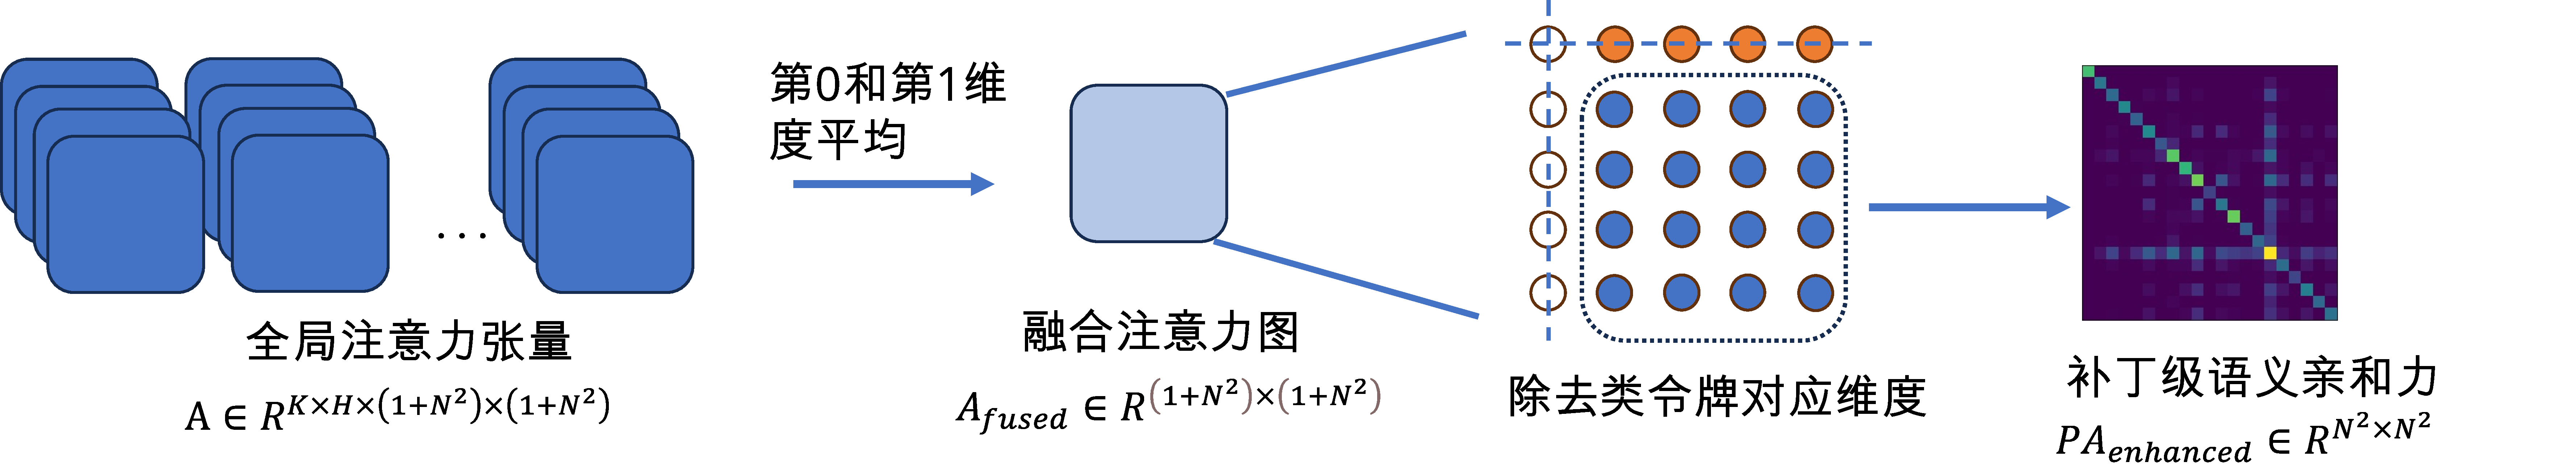
\includegraphics[width=6in]{fig/fig2.pdf}}
    \begin{CJK*}{UTF8}{fs}
        \caption{补丁语义亲和力获取流程图}\label{fig2}
    \end{CJK*}
\end{figure*}

\begin{CJK*}{UTF8}{zhhei}
    \subsection{弱监督语义分割中的ViT}
\end{CJK*}

先前的WSSS方法大多建立在CNN网络之上,存在只激活最显著区域的缺点。ViT\cite{02dosovitskiy2020image}凭借其强大的全局上下文建模能力,在WSSS任务中取得成功。TS-CAM\cite{11gao2021ts}提出借助ViT和多头自注意力的特性生成CAM,来充分利用ViT的长距离建模能力。MCTformer\cite{12xu2022multi}强调了ViT中类令牌的重要性,通过嵌入多个类令牌并强制它们学习不同类的激活图,并利用特定类别的注意力图优化CAM。AFA\cite{13ru2022learning}通过额外的模块学习多头自注意力中的语义亲和力,改善了CAM的覆盖区域,缓解了CAM难以捕捉完整的目标区域的问题。ToCo\cite{03ru2023token}通过利用ViT中间层的伪标记关系来监督最终的补丁标记,从而解决ViT的过度平滑问题。然而,先前的方法通常利用ViT中的语义亲和力优化CAM,对计算资源要求较高,且直接利用可能会给CAM带来错误和误导。且ViT中多头注意力的设计目的是为了捕捉不同依赖关系,但实践中一些注意力头往往会关注相似的区域或信息,导致不同头之间存在相似性,产生冗余。本文提出的头平均注意力融合增强模块(HAAF)通过多头平均化去除上述冗余信息,淡化可能捕捉到的噪声或者无效的注意力模式,减少单个头对特定噪声的敏感度,提高模型的鲁棒性。